\documentclass[a4paper,14pt]{extarticle}
\usepackage{geometry}
\usepackage[T2A]{fontenc}
\usepackage[utf8]{inputenc}
\usepackage[french, russian, english]{babel}
\usepackage{amsmath}
\usepackage{amsthm}
\usepackage{amssymb}
\usepackage{fancyhdr}
\usepackage{setspace}
\usepackage{graphicx}
\usepackage{colortbl}
\usepackage{tikz}
\usepackage{pgf}
\usepackage{subcaption}
\usepackage{listings}
\usepackage[colorlinks, linkcolor=blue, urlcolor=blue]{hyperref}
\usepackage{indentfirst}
\usepackage{float}
\usepackage{wrapfig}
\graphicspath{{images/}}


\makeatletter
\renewcommand{\@biblabel}[1]{#1.} 
\makeatother

\geometry{left=2.5cm}
\geometry{right=1.5cm}
\geometry{top=1.5cm}
\geometry{bottom=1.5cm}
\renewcommand{\baselinestretch}{1.5}

\newcommand{\bibref}[3]{\hyperlink{#1}{#2 (#3)}}

\renewcommand{\theenumi}{\arabic{enumi}}% Меняем везде перечисления на цифра.цифра
\renewcommand{\labelenumi}{\arabic{enumi}}% Меняем везде перечисления на цифра.цифра
\renewcommand{\theenumii}{.\arabic{enumii}}% Меняем везде перечисления на цифра.цифра
\renewcommand{\labelenumii}{\arabic{enumi}.\arabic{enumii}.}% Меняем везде перечисления на цифра.цифра
\renewcommand{\theenumiii}{.\arabic{enumiii}}% Меняем везде перечисления на цифра.цифра
\renewcommand{\labelenumiii}{\arabic{enumi}.\arabic{enumii}.\arabic{enumiii}.}% Меняем везде перечисления на цифра.цифра

\newcommand{\imgh}[3]{\begin{figure}[h]\center{\includegraphics[width=#1]{#2}}\caption{#3}\label{ris:#2}\end{figure}}

\begin{document}
	\begin{titlepage}
\newpage

\begin{center}
Федеральное государственное автономное образовательное учреждение высшего образования "Национальный исследовательский университет "Высшая школа экономики"
\\
\medskip
Факультет компьютерных наук \\
Основная образовательная программа \\
Прикладная математика и информатика \\
\end{center}

\vspace{8em}

\begin{center}
\Large КУРСОВАЯ РАБОТА \\
\end{center}

\vspace{2em}

\begin{center}
\textsc{\textbf{
Исследовательский проект на тему
\linebreak
"Оценка неопределенности для Машинного Перевода"}}
\end{center}

\vspace{6em}



\newbox{\lbox}
\savebox{\lbox}{\hbox{Ментимер Шаймиев Рудольф Нуриев}}
\newlength{\maxl}
\setlength{\maxl}{\wd\lbox}
\hfill\parbox{17cm}{
\hspace*{5cm}\hspace*{-5cm}Выполнил студент группы 171, 3 курса: \hfill Кузнецов Дмитрий Сергеевич\\
\hspace*{5cm}\hspace*{-5cm}Руководитель КР\hfill 
научный сотрудник Лобачева Екатерина Максимовна\\
%\hspace*{5cm}\hspace*{-5cm}Куратор:\hfill < степень>, <звание>, <ФИО полностью>\\
}


\vspace{\fill}

\begin{center}
Москва 2020
\end{center}

\end{titlepage}% это титульный лист
	\newpage

	{
		\hypersetup{linkcolor=black}
		\tableofcontents
	}

	\newpage
	
	\section{Annotation}
	In machine translation, there is a significant problem of improving the quality of models. There are now many studies on the topic of uncertainty estimation. However, there is no almost works on uncertainty estimation in neural machine translation. In this paper, we will study the relationship between uncertainty and the quality of machine translation models.
	\section{Keywords}
		machine translation, uncertainty estimation, beam search, larger beam size problem, model uncertainty, data uncertainty
		
	\section{Introduction}
	Nowdays machine translation is one of the most popular areas of machine learning. There are two fundamental approaches to solving this problem: statistical and neural machine translation. In the first case, classical approaches of classical statistical machine learning are used, in the second - modern technologies of deep learning. As in any field, there are a lot of actual unresolved problems in machine translation. In particular, in contrast to statistical machine translation, in neural machine translation  quality of prediction degradation appears with a hypothesis search width increase.
	
	Another relatively modern area in machine learning is uncertainty estimation. Using the methods of uncertainty estimation it is possible to build metrics for confidence in predictions of models. There are several types of uncertainties. Some of them are caused by certain artifacts in the data, while others are caused by the model's ability to understand the proposed data. In any case, the uncertainty estimates indicate that the model is doubtful about making certain predictions.	
	
	In this paper, we study the correlation between machine translation model errors and uncertainties in both data and models. We propose an approach to using uncertainty estimation as a way to improve the quality of the model or architecture.
	\section{Machine Translation}
	\subsection{Preliminary}
		The task of machine translation is to provide a sentence equivalent in meaning in the target language for the original sentence in the source language. Let $e_1, \dots, e_n$ be a sequence of input sentence tokens' vector representation in the source language. The machine translation model is required to build a sequence of tokens $f_1, \dots, f_m$ in the target language, moreover, in this language, this sequence must have the original meaning.
	
	Most modern neuromachine translation models follow the paradigm \bibref{seq2seq}{Sutskever et al.}{2014} (seq2seq). Seq2seq models often consist of two recurrent neural networks or groups of networks. One network that processes input tokens is called \textit{encoder}, the second network that builds output predictions is called \textit{decoder}. The encoder task is to encode the input sequence into some hidden representation $h_1, \dots, h_p$, which is fed to the decoder as hidden initialization before building the output prediction. The decoder output is a vector set $\{(p_{i1}, \dots, p_{id})\}_{i=1}^{m}$, where $d$ - target language dictionary power, $m$ - maximum possible prediction sequence length, $p_{ij}$ - the model's confidence that the $i$th token of the predicted sentence will be the $j$th token from the target language dictionary. As a result, the translation model builds a "probability distribution" in the space of the cartesian product of the target dictionary.

	The simplest and most obvious way to build a prediction (final translation) is to select the token that the model is most confident in at each step. If $f_1, \dots, f_m$ is a sequence of model hypotheses' tokens, then $f_i := argmax \, \{p_{ij}\}_{j=1}^{d}$. However, for an optimal prediction $f_1^*, \dots, f_m^*$ it is not always true that in terms of model confidence $f_i^* = argmax \, \{p_{ij}\}_{j=1}^{d}$. This phenomenon is also related to the beam problem, which we will discuss in more detail in the following chapters.
	\subsection{Statement}
	First of all, let's define the concept of \textit{embeddings}. Embeddinges are some numerical vectors of a special vector space that bijective correspond to words from the dictionary of a certain language. Then consider the following statement.
Let $\textbf{x}, \textbf{r}$ be embeddings corresponding to the input and output tokens $\textbf{e}, \textbf{f}$, respectively.
Then the machine translation model sets the following cumulative probability:
	\begin{equation}
		P(\textbf{y} | x, \theta) = P(y_1 | x, \theta) \prod_{i=2}^{L} P(y_i | y_{<i}, \textbf{x}, \theta)
	\end{equation}
	
	Here $\textbf{y}$ is a certain sequence of tokens that corresponds to the translation from the model's point of view. $y_{<i}=(y_1, \dots, y_{i - 1})$ , and $\theta$ is machine translation model parameters that are configured during training.

	Based on these probabilities, a model selects the final embedding sequence $\textbf{y} = (y_1, \dots, y_m)$ and it bijective restores the final tokens $\textbf{h} = (h_1, \dots, h_m)$. As we discussed earlier, the deciding rule can be a greedy choice, i.e. at each iteration, an embedding is selected with the maximum conditional probability of $P (y_i | y_{<i}, \textbf{x}, \theta)$. Some other approach can be used as the deciding rule, such as beam search, which we will discuss later.
	
	For simplicity, due to bujection, we will further understand tokens as tokens embedding, and we will implicitly mean transferring to the final tokens space. Therefore, our final notation will be: $X = (x_1, \dots, x_n)$ - set of all sentences in the source language, $R = (r_1, \dots, r_n)$ - set of reference translations in the target language. $Y = (y_1, \dots, y_n)$ - a set of translations from the point of view of our model.

	The most common quality measure in a machine translation problem is BLEU.
	
	Let the model for some pair of sentences be $\textbf{x}, \textbf{r}$ built a translation of $\textbf{y}$.
	\begin{equation}
		BLEUK = \min\Big(1, \, \frac{|\textbf{y}|}{|\textbf{r}|}\Big) \big(\prod_{i=1}^{K} precision_i\big)^{\frac1K}
	\end{equation}

	Here, $precision_i$ means $precision$ calculated for all i-grams.
	\section{Beam Search}
	\subsection{Motivation}
	Beam search is used as a more effective solution for building predictions. Its main idea is that instead of selecting the most likely token at each step, we require the model to store $b$ the most likely predictions' prefixes $y_{b1}, \dots, y_{bt}$. Using this approach, we do not choose the locally optimal token, but in general the optimal prefix, which will increase the chances of building a correct prediction.

	It is easy to understand that with the increase of $b$ (this hyperparameter is called \textit{beam size}), the quality of the prediction should also increase, since the number of greedy searches is growing. In practice, it turns out that in neuromachine translation, starting from a certain threshold, the quality decreases significantly with increasing beam size. An illustration of this phenomenon can be seen in Fig. 1. The model used in the experiment is described in the  \bibref{fconv}{Jonas Gehring}{2017}. 
	
	\begin{figure}[t]
		\center{
			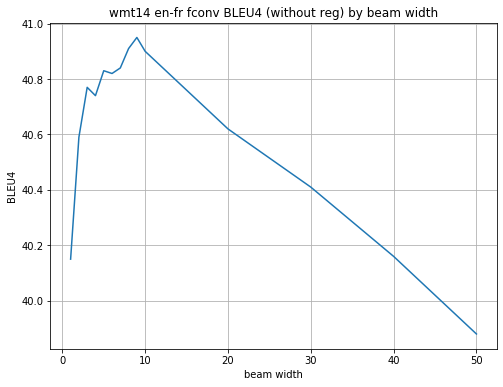
\includegraphics[width=0.7\textwidth]{fconv-bleu4.png}
		}
		\center{\caption{Convolutional Sequence to sequence model BLEU4 evaluation by beam size. Training set: \textit{WMT'14 English-France}}}
	\end{figure}
	
	This problem is called \textit{larger beam size problem}. Next, we will look at the possible causes of this phenomenon in details, until we note that the following situation is not excluded. Suppose on $k_1$ iteration step beam search stores the prefix $y_1, \dots, y_{k_1}$ among $b$ locally optimal, which has the least model confidence among all $b$ prefixes. Let this prefix be constructed in such a way that on the next steps model will find a suffix that complements it in such a way that the final sentence is considered the optimal translation from the model's point of view. There are cases when such a translation can be incorrect. Consider following example. Let us train a translation model on a fairy tale corpus, the source language is Russian and the target language is English. Consider the following sentence: \textit{Жульничество на экзамене однажды может закончиться проблемами}. Suppose following sentence is a model prediction: \textit{At the examination once upon a time}. It is obvious that the meaning of the translation does not correspond to the original sentence, but this sentence is optimal from the point of view of our hypothetical model. Beam problem can cause such situations. The prefix \textit{At the examination once} may have been included in a broad beam search and have been earned a low model confidence. However, due to the fact that we train on a large corpus of fairy tales, where there are many examples of sentences like \textit{Once upon a time...} our model decides that after \textit{Once} it is probably to continue prefix with suffix \textit{upon a time}, which lead to a bad translation.
	\subsection{Method definition}
	Suggest $k$-long prediction prefix:
	\begin{equation}
		y_{<k}^{i} := (y_1^{i}, \dots, y_k^{i}) \text{, \,\, where i - beam search branch index}
	\end{equation}
	
	Let us introduce following iterative method:
	
	\begin{enumerate}
		\item Let us submit a special token of the beginning of the sentence and the encoder hidden state to the decoder input. We get a certain tokens' confidence vector $(p_1^{00}, \dots, p_d^{00})$, where $d$ - target dictionary power.
		
		\item Take tokens whose confidence values are $beam$ highest among $ (p_1^{00}, \dots, p_d^{00})$. Here $beam$ is the hyperparameter of the method and is called \textit{beam size}. As a result, we will remember: $y_{<1}^1, \dots, y_{<1}^{beam}$. 
		
		\item In the next iteration, we will submit to the decoder $(y_1^{00}, \dots, y_d^{00})$ as inputs and the hidden state of the previous step. For each token, we get our output distribution $(p_1^{1i}, \dots, p_d^{1i})$ (here $1$ is the iteration number, $i$ is the token number).
		\item For all token $i \in \overline{1, beam}$ consider $\forall j \in \overline{1, d}: \,\, p(f_{:1}^i) * p_j^{1i}$. We get a set of prefixes of length $2$. Let us choose among all $beam * d$ prefixes $beam$ with the greatest confidence. Remember them: $y_{<2}^1, \dots, y_{<2}^{beam}$
		
		\item Iteratively, we will continue the operation $\forall k \in \overline{3, m}$. 
		
		We will get: $y_ {<k}^1, \dots, y_{<k}^{beam}$
		
		\item As the final prediction select $y_{<m}^i, \dots, y_{<m}^i$ such that its confidence is greatest $\forall i \in \overline{1, beam}$
	\end{enumerate}
	
	In summary, this method stores $beam$ of the "most likely" prefixes at each decoding iteration, in contrast to the naive approach, which greedily selects 1 locally optimal hypothesis at each iteration.
	
	\subsection{Large Beam Size Problem}
	In General, in neuromachine translation tasks large beam size problem is a phenomenon, as a result of which, starting from a certain threshold value, the quality metric decreases with the growth of the beam size. In this section, we will look at some approaches that do not solve the problem completely, but significantly reduce the effect of metric degradation.
	
	The article \bibref{corr_len_bias}{Murray et al.}{2018} raises two issues: the beam problem and the tendency of NMT models to make short predictions. According to the author, solving the short prediction problem involves solving the beam problem.
	
	As a demonstration of the reasons listed in this article that cause the beam problem, consider the following example from the article.
	
	On the Fig.2. we can see a tree of Beam Search predictions for the word \textit{un hélicoptère}. Let the size of the beam search be 2 and on the first iteration we saved two hypotheses: \textit{a} and \textit{an}. Note that all 4 following hypotheses can be potential translation options, but \textit{a helicopter} in this example is a correct translation. However, \textit{autogyro} is an only one continuation for prefix \textit{an}, thefore the model confidence for this suffix is $1$, and as a result, the model confidence to predict \textit{an autogyro} is equal to $0.4$. At the same time, the probability mass for the \textit{a} continuation suffixes is divided among the words: \textit{helicopter, chopper, whirlybird}. As a result, the confidence for the correct translation of \textit{a helicopter} from the model's point of view is $0.36$. As a result, the model will give a bad prediction. Larger beam size we take, higher probability we get in this situation, hence the loss of quality.
	
	\begin{figure}[t]
		\center{
			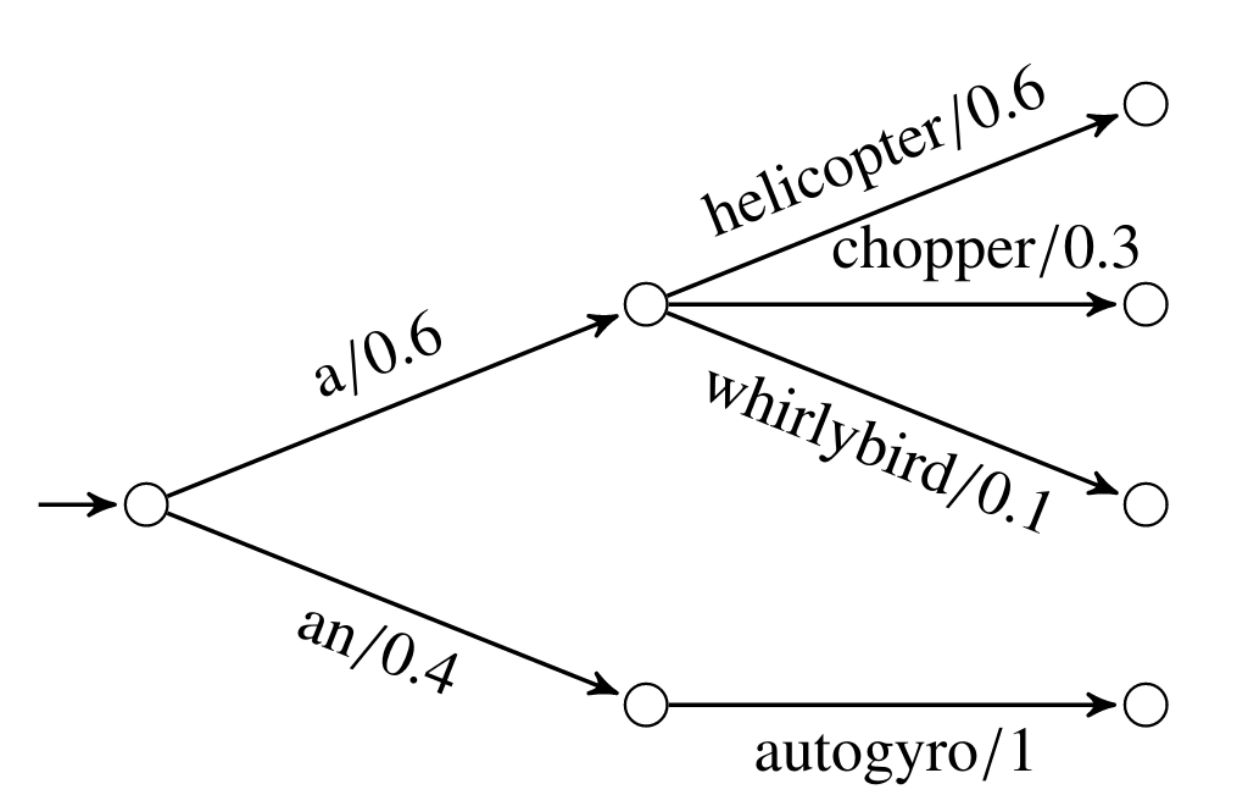
\includegraphics[width=0.5\textwidth]{helicopter.png}
		}
		\center{\caption{Label bias causes this toy word-by-word translation model to translate French helicopter incorrectly. This figure is taken from [4].}}
	\end{figure}
	
	Note that this example demonstrates the fact that if a certain prefix involves a low-entropy suffix, the model tends to ignore the second input token and predict with high confidence one of several highly probable low-entropy suffixes. As a result, the low entropy of the suffix leads to overestimation of this prediction branch and as a result, poor quality. In addition, there is a high probability of getting short predictions due to low entropy, since the model begins to ignore some tokens in favor of high confidence of low-entropy suffixes. For this reason, the authors of the article consider the short prediction problem and the beam problem together.
	
	Standard quality functional for a machine translation task is \textit{cross-entropy}:
	\begin{equation}
		s(\textbf{y}) = \sum_{i=1}^{L}\log p(y_i | y_{<i}, \textbf{x}, \theta), \,\,\, \text{where $L$ - translation length}
	\end{equation}
	
	The authors consider the following quality functional adjustments as solutions:
	\begin{enumerate}
		\item Length normalization
		\begin{equation}
			s'(\textbf{y}) = s(\textbf{y}) / L
		\end{equation}
		
		\item \bibref{gnmt}{Google's NMT system}{2016}. Length normalization. 
		\begin{equation}
			s'(\textbf{y}) = s(\textbf{y}) \Big/ \frac{(5 + L) ^ \alpha}{(5 + 1) ^ \alpha}
		\end{equation}
		
		\item Word reward
		\begin{equation}
			s'(\textbf{y}) = s(\textbf{y}) + \gamma L
		\end{equation}
	\end{enumerate}
	
	Let us look at the results presented in the article for the \textit{WMT'17 Russian-English} model. The architecture presented in the article \bibref{encdec_att}{Bahdanau et al.}{2015} was chosen as the baseline. Appealing to experiments results from the paper we observe that the solution of the short prediction problem using methods proposed above significantly decreases the influence of the beam problem on the considered dataset. Comparing \textit{word reward} and {length normalization}, we can see that they earn quite close BLEU values and lager beam size problem affects models in a same way, when baseline model suffers from beam problem significantly.
	
	Let us now look at the article \bibref{six_chall}{Koehn et al.}{2017}. This is a review article on the main problems of neuromachine translation, including the beam problem.
	
	The authors of the article do not present new solutions for the problem, but conduct a review study. As a baseline, they use the same neural network as in the previous article: attention-based encoder-decoder. Fig. 3 presents their results for various \textit{WMT} datasets. Here, normalization is the Length normalization from the previous article.
	
	\begin{figure}[t]
		\center{
			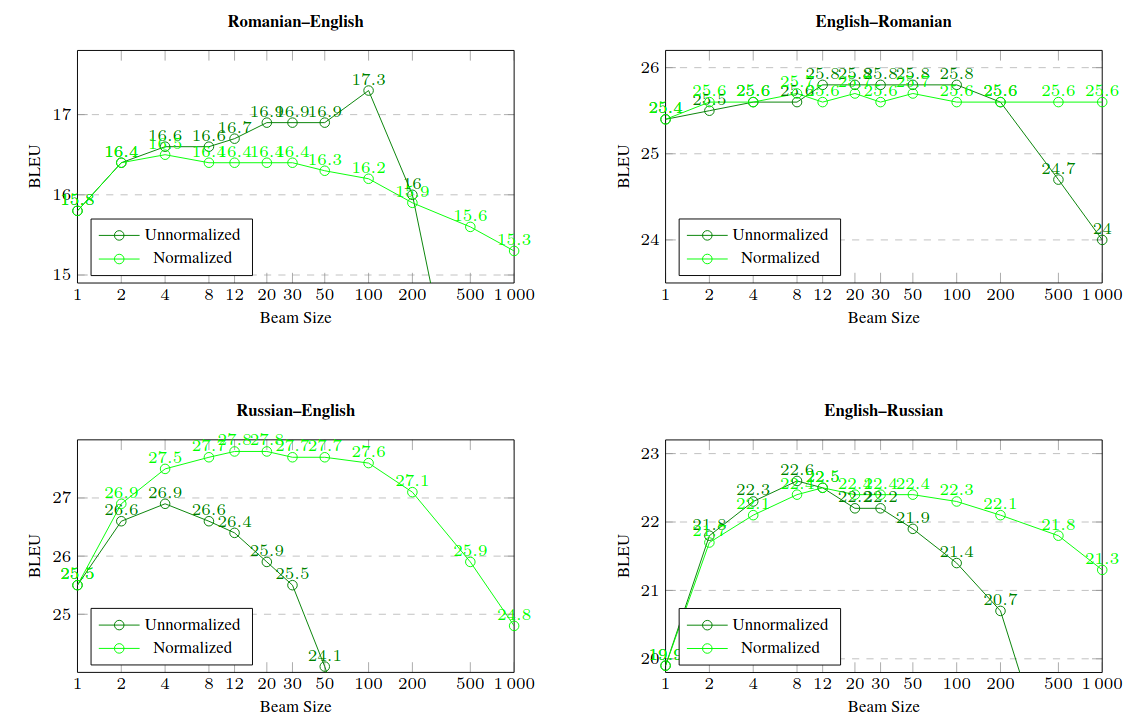
\includegraphics[width=0.8\textwidth]{six_chall_graph.png}
		}
		\center{\caption{Translation quality with varying beam sizes. For large beams, quality decreases, especially when not normalizing scores by sentence length. This figure is taken from [7].}}
	\end{figure}
	
	The results obtained in this article are consistent with the results and conclusions of the previous article.
	
	Consider an article that offers a different method for solving the problem \bibref{calibration}{Kumar et al.}{2019}.

	In this article the beam problem solution is based on the calibration of the probability distribution $p_{it}: = p(y_{i, t} | y_{i,<t})$, here $i$ is the index of the sample example. Before starting the review, let us introduce the definition of "well-calibrated" distribution. Output distribution $p (y_{i, t} | y_{i, <t})$ \textit{well calibrated} if:
	\[
		\forall \beta \in [0, 1]: \frac{ | \{ y \in V |\, p(y) = \ beta \} | }{d}=\beta
	\]
	where V is the target language dictionary.
	
	Let us denote calibration metrics \textbf{expected calibration error (ECE)}:
	
	Let $\mathbf{r}_i = (r_{i1}, \dots, r_{im})$ be reference sentece $\mathbf{x}_i$.
	
	Model predictions: $\mathbf{y}_{it} := argmax_{y} p(y | y_{i, <t})$.
	
	$C_{it}(f) := \delta(r_{it} = y)$, where $\delta$ - Kronecker delta.
	
	Let us divide probability space $[0, 1]$ by $M$ equal bins: $I_1, \dots, I_M$.
	
	Let $L = \sum_i^N |\mathbf{r}_i|$ be a total output token length.
	
	Then:
	\begin{equation}
		ECE = \frac1{L}\sum_{b=1}^{M}\Big|\sum_{i, t:\, p(\mathbf{y}_{it}) \in I_b} C_{it}(\mathbf{y}_{it}) - p(\mathbf{y}_{it})\Big|
	\end{equation}
	
	The reasons why the probability distribution calibration can solve problems with beam size follow from the examples we discussed above.
	
	The authors consider the classic \textit{temperature scaling as the basic method}:
	
	The method is quite simple. It is necessary to raise all probability distribution to the power of $\frac1{T}$, where $T$ is the hyperparameter of the method:
	\[
		p_{it} \rightarrow p_{it}^{\frac1{T}}
	\]
	
	This approach does not change the relative values of probabilities, i.e. it does not locally change the optimality of a particular choice, but it helps to smooth out the consequences of overestimating or underestimating certain prefixes or suffixes.
	
	The authors consider 3 models trained on \textit{WMT} as a baseline: \bibref{encdec_att}{attention-based encoder-decoder}{2015}, GNMT \bibref{gnmt}{Wu et al.}{2016}, transformer \bibref{transformer}{Vaswani et al.}{2017}. Authors build probability plots for each model output distribution with and without classic temperature scaling. Results show that transformer model output distribution is closer to perfect calibration than other models, even without scaling. Classic attention-based encoder-decoder, trained on English-Vietnamese WMT dataset, shows the worst calibrated output distribution without using temperature scaling. Other model in a list, trained on other sets of data, shows quite similar results without calibration method and with temerature scaling, this results differ a little from transformer values. Graphs show that using classic temperature scaling probability plot goes to perfect, ECE decreases even in the worst case scenarios. 
	
	In order not to overweight the literary review, we will not formally introduce the method proposed by the authors. We will consider conceptual differences from the default temperature scaling. To study the formal definition of the method, you can refer to the article \bibref{calibration}{Kumar et al.}{2019}.
	
	As a result of experiments, the authors found out that end of sequence (EOS) token probability is the worst calibrated among all other tokens. Therefore, first of all, the authors calibrate the distribution of the EOS token. This observation strongly correlates with the conclusions from the articles reviewed earlier. In contrast to the classic temperature scaling and the hyperparameter selection on a validation set, the authors propose to make the hyperparameter flexible, different for each example and token index, i.e. not to smooth the entire probability mass, but to smooth it depending on the offset of the probability density on the token. To find the values of hyperparameters, it is proposed to use two fully connected two-layer neural networks with 3 neurons on the hidden layer. The composition of two neural networks with optimization \textit{Negative Log Likelihood (NLL)} is proposed to train to predict the value of the hyperparameter $T$ for a given example and a token in the prediction.
	
	Authors present experiments results, that comparing ECE and BLEU for baseline models with authors calibration method, classic temperature scaling and without any calibration. In generall we can say that temperature scaling gives significant fall comparing to models without any calibration (about several points of number). Authors' calibration method shows the best results except only one case, ECE of output distribution is less than ECE of temperature scaling models (about several points of number after the dot). It can also be seen that the authors' calibration method achieves the best results on the most part of the baseline models from the BLEU point of view.
	
	Now, turning to Fig. 4, let us look at the effect of the authors' calibration on the beam size problem. It is easy to see that calibration significantly reduces the impact of the beam problem.
	
	\begin{figure}[t]
		\center{
			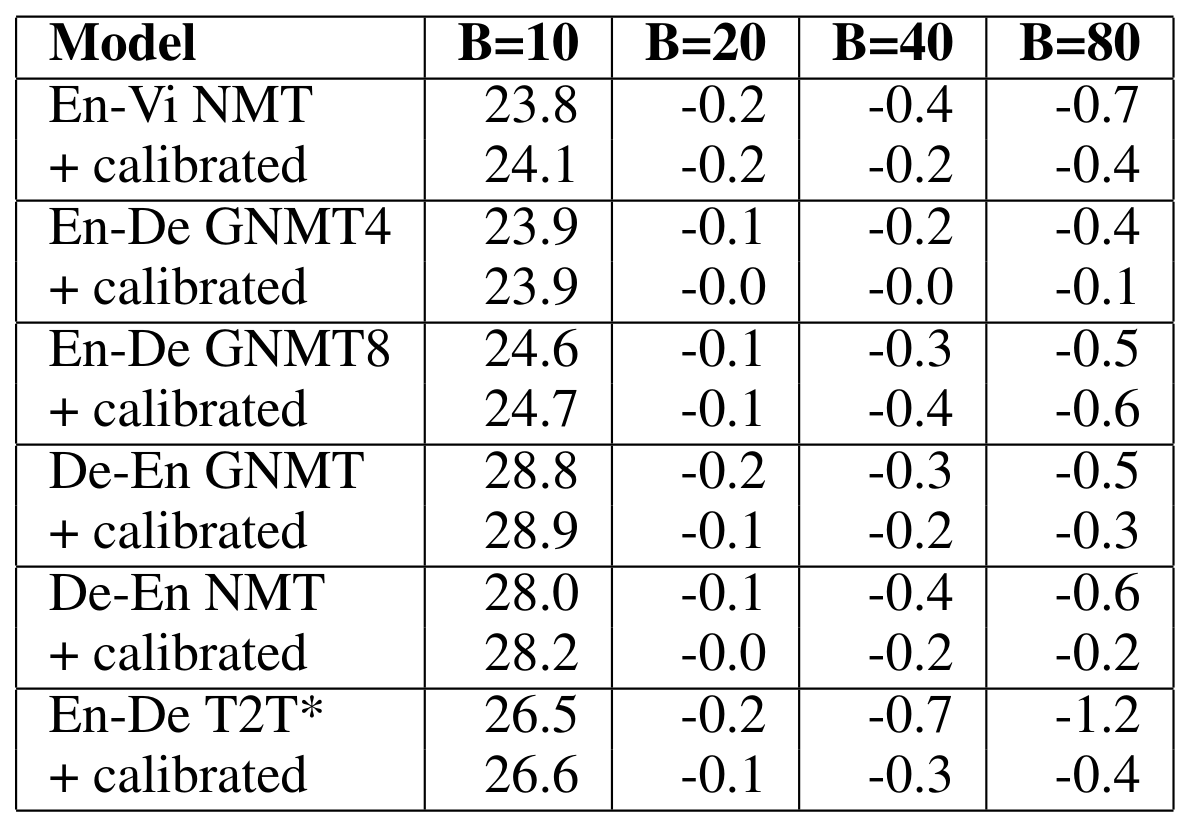
\includegraphics[width=0.6\textwidth]{beam_calibration.png}
		}
		\center{\caption{BLEU with increasing beam on the devset. *Beam sizes for Transformer/T2T: 4, 8, 10 and 12. This figure is taken from [8].}}
	\end{figure}
	
	In this section, we investigated the possible causes of the beam problem, as well as methods of counteraction. Unfortunately, it is not possible to draw unambiguous conclusions from the results of the article about which method shows the best results due to the fact that the experiments in the articles were carried out in different configurations. According to approximate estimates, both methods show good results, are easy to implement, but do not solve the problem completely.
	
	\section{Uncertainty}
	\subsection{Definition}
	This information was obtained from the article \bibref{prior}{Malinin et al.}{2018}
	
	Uncertainty in machine learning is usually understood as a measure of the nondegeneration of the distribution on the model predictions at a fixed input. Less formally, if we were able to estimate uncertainty, we could tell how much we can trust the model's predictions.
	
	There are several types of uncertainties: data uncertainty, model uncertainty, and distributive uncertainty. \textit{Data uncertainty (aleatoric uncertainty)} - type of uncertainty caused by the nature of the data, including noise, class balance, etc. \textit{Model uncertainty (epistemic uncertainty)}  measures uncertainty caused by a model specifity, how good a model understands given data. \textit{Distributional uncertainty} measures similarity between training and test data, caused by unknown or strange test examples. 
	
	It is important for the model to evaluate all types of uncertainty, because they are caused by different reasons and have different negative effects.
	
	\subsection{Analyzing Uncertainty in Neural Machine Translation}
	In the article \bibref{anal_uncertainty}{Ott et al.}{2018} \textit{data uncertainty} is being investigated.
	
	Let us introduce several base definition from the article. \textit{Intrinsic uncertainty} is the result of existence of several semantically equivalent translations of the same source sentence, for instance there are several ways to express the same meaning. Also situations when target language is more complex than a source language, it can cause an uncertainty. In such situations it could be impossible to earn additional information, such as gender or tense, which is necessary to build correct prediction in a source language. Web data crawling to construct train corpus can cause \textit{extrinsic uncertainty}. For example, authors notice that at least 1\% sentences in WMT datasets is just a copy of a source sentences.
	
	The architecture described in the article \bibref{fconv}{Gehring et al.}{2017} is specified as the baseline of the experiments.
	
	One of the main problems that is raised in this article is an effect of \textit{uncertainty} on the degradation of quality with the growth of beam size. Authors notices copies (extrinsic uncertainty) are overrepresented in the output of beam search. Also they say that bigger beam size we take, more copies appear in a beam search tree, and this growth is quite significant.
	
	\begin{figure}[t]
		\center{
			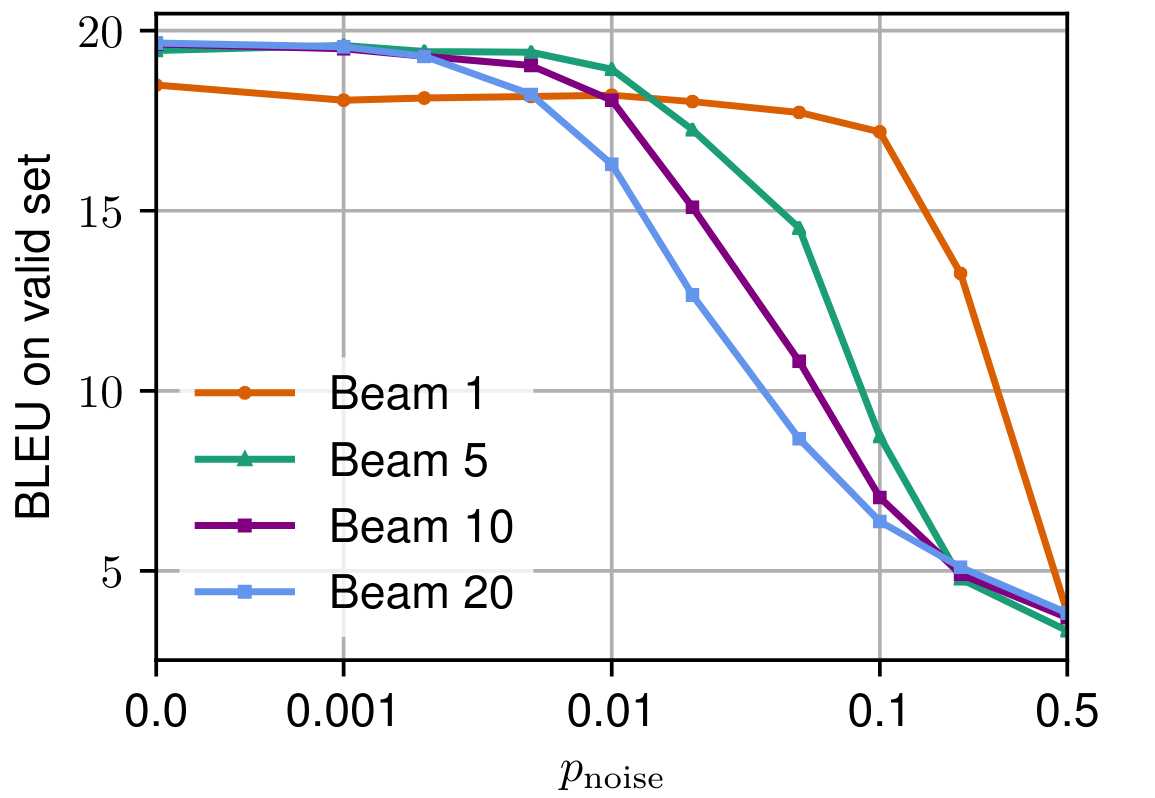
\includegraphics[width=0.6\textwidth]{unc_beam_noise.png}
		}
		\center{\caption{Translation  quality  of  models  trained  on  WMT’17 English-German news-commentary data with added synthetic copynoise in the training data (x-axis) tested with various beam sizeson the validation set. This figure is obtained from [9].}}
	\end{figure}
	
	The authors conducted an experiment, the results of which can be seen in Fig. 5, in which WMT'17 added explicitly replaced random examples from the training with copies of the original sentence. It is clearly seen that this leads to quality degradation with increasing noise. Moreover, models with a larger beam size suffer more from extrinsic uncertainty, which confirms the thesis put forward in the previous paragraph.
	
	The authors suggest two approaches to preparing data for training. First, they remove train examples, which has low score in a model trained on the news-commentary part of WMT'17 En-De point of view (filtered). Second, they restrict beam search hypotheses, which has BLEU with source sentence more than 50\% (no copy). The results can be seen in Fig. 6. They are fully consistent with the conclusions obtained earlier.
	\begin{figure}[H]
		\center{
			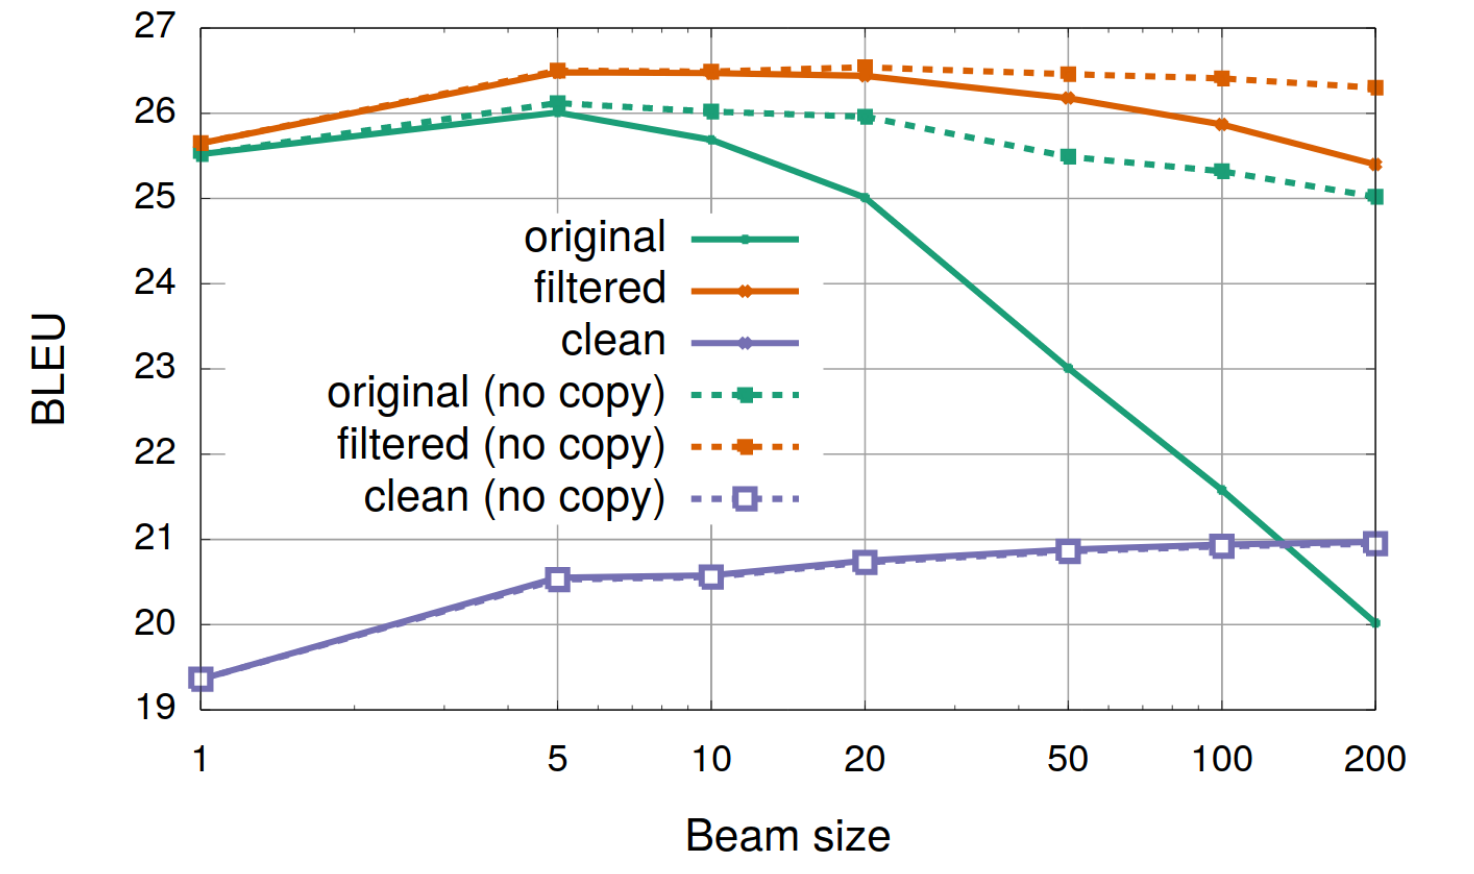
\includegraphics[width=0.6\textwidth]{unc_beam_meth.png}
		}
		\center{\caption{BLEU on newstest2017 as a function of beam width for models trained on all of the WMT’17 En-De training data (original), a filtered version of the training data (filtered) and a small but clean subset of the training data (clean). They also show results when excluding copies as a post-processing step (no copy). This figure is obtained from [9].}}
	\end{figure}
	\subsection{Ways of uncertainty estimation}
	In this section, we will refer to the article \bibref{uncertainty}{Malinin et al.} {2020}, which discusses various approaches to estimating uncertainty for structured predictions and some its applications. In this section, we will consider problems in which solutions are described by the probabilistic model (1).

	The author identifies two main approaches to estimating uncertainties for structured predictions: sequence-level and token-level. In the case of sequence-level, the uncertainty is estimated in the space of final predictions (the Cartesian product of the dictionary). In the case of token-level, the uncertainty is evaluated at the level of individual sequence tokens (the dictionary space). Estimating uncertainties at different levels allows us to solve different types of problems.
	
	The main tool for estimating uncertainty in the article is the use of models ensemble from a certain parametric family of models $\mathcal{F}(\theta)$ , where $q(\theta)$ - an empirical estimate of a prior distribution of models $p(\theta)$. Informally speaking, the following idea is a prerequisite for using ensembles. If many different models from the same family vote for the same verdict, it is highly probable that we can trust this verdict. In the opposite situation, if the models are not consistent in their predictions, this observation can become an indicator of uncertainty, in particular, it may indicate that the presented problem is out of the general pattern of the data that the models were able to train in their generality.

	The starting point for entering uncertainty estimation in the article is the following relation:
	\begin{equation}
		\underbrace{\mathcal{I}[y, \theta|\textbf{x}, \mathcal{D}]}_\text{Knowledge Uncetainty}
		= 
		\underbrace{\mathcal{H}[P(y | \textbf{x}, \mathcal{D})]}_\text{Total Uncertainty}
		-
		\underbrace{\mathbb{E}_{q(\theta)}[\mathcal{H}[P(y| \textbf{x}, \theta)]]}_\text{Data Uncertainty}
	\end{equation}
	
	Here $\mathcal{H}$ is Shannon entropy and $\mathcal{I}$ - mutual information.
	
	Knowledge uncertainty can also be evaluated using a different metric suggested in the article, which correlates with the one already considered:
	\begin{equation}
		\mathcal{K}[y, \theta] = \mathbb{E}_{q(\theta)q(\hat{\theta})}[
			\mathrm{KL}[P(y|\textbf{x}, \theta) || P(y|\textbf{x}, \hat{\theta})
		]
	\end{equation}
	
	We have considered only a small part of the uncertainty metrics proposed by the author. The full study can be found in the original article. We will discuss the metrics described above in more detail in the following chapters.

	Malinin in his work presents some experiments demonstrating the effectiveness of uncertainty estimation by these methods at various estimation levels for the ASR problem. In particular, experiments: out of distribution detection and misclassification detection. However, this article does not deal well with uncertainty estimation for a machine translation problem.
	\section{Overview summary}
	We have reviewed work workaround. In this paper, we plan to study the correlation between uncertainty and translation errors. In particular, we want to find out how to improve the quality by adding some knowledge about the uncertainty of prediction to the model. Due to the fact that the token-level estimation for the machine translation task is poorly understood, we will consider this approach. We will also try to find out the correlation between the uncertainty estimation and the larger beam size problem.
	

\section{Preliminary}
	Recall the workaround of our work.

	Let $X = (x^1, \dots, x^N)$, $R = (r^1, \dots, r^N)$ a parallel corpus of sentences, where $X$ corresponds to the source language, and $R$ corresponds to the target language (the one we are translating to). The final translation of a certain sentence $x$ is based on the following probabilistic model (our model of neuromachine translation):
	\begin{equation*}
		P(\textbf{y} | x, \theta) = P(y_1 | x, \theta) \prod_{i=2}^{L} P(y_i | y_{<i}, x, \theta)
	\end{equation*}
	
	The purpose of this work is to use uncertainty estimation (total, knowledge) to determine situations when the model makes an error in predicting the next token $y_i$. We will look at several approaches and ways to use them.

	The baseline model of this work is the transformer \bibref{transformer}{Vaswani et al.} {2017}, implemented in the fairseq Facebook library. Next, in all experiments, we will consider an ensemble of 5 transformers. The final probability model of the ensemble has a form:
	\begin{equation*}
		P(y_i | y_{<i}, x, \mathcal{D}) = \frac1{K} \sum_{j=1}^{K}P(y_i | y_{<i}, x, \theta_j)
	\end{equation*}
	
	In our case, $K=5$. Each model in the ensemble was trained on shared data $X, R$, but from different initialization points.

	\textit{IWSLT`14 De-En} was taken as a training, test, and validation samples for transformer models. The target metric for this work is \textit{BLEU4}.

	The final graph of the results can be seen at image 7.
	
	\begin{figure}[t]
		\center{
			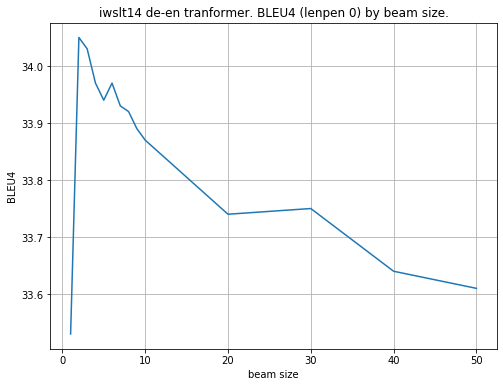
\includegraphics[width=0.6\textwidth]{images/single_transformer_bleu.png}
		}
		\center{\caption{BLEU on test set for transformer model by beam size}}
	\end{figure}
	
	An ensemble of 5 models with the \bibref{fconv}{Gehring et al.}{2017} architecture was also trained. The transformer showes higher results, so we will consider the transformer as the final model for experiments.
	
	The configuration of each model in the ensemble of transformers was as follows:
	\begin{enumerate}
		\item $clip\_norm = 0$
		\item $learning\_rate=5*10^{-4}$
		\item $label\_smoothing=0.1$
		\item $epochs=75$
		\item $lenpen=0$ (We want to know how uncertainty estimation will affect Bleu degradation by beam size)
	\end{enumerate}
	
	The graphs of the final metrics show that with the growth of beam size BLEU degrades. As we found out earlier, this can be caused by overestimating or underestimating the probabilities of certain tokens. In this paper, we will also try to identify the correlation of this problem with the uncertainty.
	
\section{Misclassification detection}
	In \bibref{uncertainty}{Malinin et al.} {2020}, an attempt to detect falsely predicted tokens on the ASR problem is considered. Unfortunately, the author did not conduct a similar experiment for NMT due to the complexity of defining the correct target metric in machine translation.

	In our work, we decided to explicitly check whether some uncertainty estimates can detect false predictions of the next token.

	The structure of the experiment will be as follows. We consider the corpus of sentences $X, R$. Let $y = (y^1, \dots, y^N)$ - corresponding translations constructed by the ensemble. Let $r_{i}, y_{i}$ be $ith$  true translation and model translation tokens, respectively. Enter the following indicator of the ith token correctness in translation:
	\begin{equation}
		correct(y^{i}, \textbf{r}) := [y^{i} \in \textbf{r}]
	\end{equation}
	
	This indicator value will be our target function, which we want to predict based on the uncertainty estimation. Malinin introduces the \textit{total uncertainty estimation}:
	\begin{equation}
		TU(y_i) := \mathcal{H}[P(y_i|y_{<i}, \mathcal{D})]
	\end{equation}
	
	Here, the Shannon entropy is considered as $\mathcal{H}$. This metric does not separate the types of uncertainties that we have discussed earlier, it is an indicator for any manifestation. It shows how much the probability mass of the final ensemble is sparse by dictionary tokens.

	Then for each $y_i^j \in H$ token, we have the target functions $correct(y_i^j, r^j)$ and uncertainty estimates $TU (y_i^j)$. We scale the uncertainty estimates to $[0, 1]$ and get some model that predicts confidence in the error of a particular token prediction.
	
	\begin{figure}[t]
		\center{
			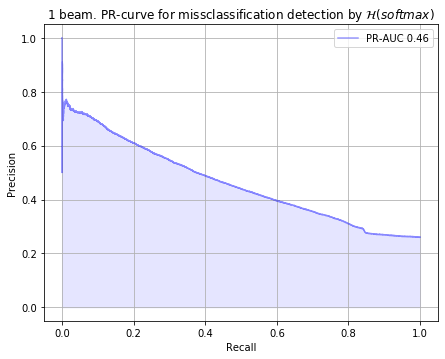
\includegraphics[width=0.6\textwidth]{images/malinin_in_tu.png}
		}
		\center{\caption{PR-curve for misclassification detection by TU}}
	\end{figure}
	The results of the experiment can be seen in image 8. If we try to maximize the F1-score, results turned out to be worse than the random predictor. However, if we are intresting only in a small percentage of errors, we can get a relatively good detection accuracy.

	The results obtained by us are consistent with the thesis put forward by Malinin. It would seem that we have fixed easy correctness indicator (any token that is not in the translation at all is marked as an error), but the uncertainty estimation works worse than a random prediction. The problem lies in the fact that if the translation is a close meaning synonym, in which the ensemble models are strongly confident, then from the point of view of our indicator - this is an error, but the uncertainty estimation will not detect any anomalies. As noted by Malinin in his article, the solution to the problem will be human manual data markup to identify more meaningful targets in this experiment.

	However, we will still try some other approaches and try to compare them with the current. We may be able to use other ratings or similarity indicators to achieve higher quality.
	
	Malinin considers another way of uncertainty estimation:
	\begin{equation*}
		\mathcal{K}[y, \theta] = \mathbb{E}_{q(\theta)q(\hat{\theta})}[
			\mathrm{KL}[P(y|\textbf{x}, \theta) || P(y|\textbf{x}, \hat{\theta})
		]
	\end{equation*}
	
	\begin{figure}[t]
		\begin{subfigure}{.45\textwidth}
			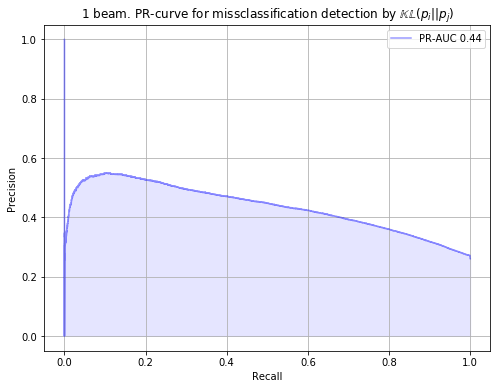
\includegraphics[width=\textwidth]{images/malinin_in_kl.png}
			\center{\caption{$\mathcal{K}[y, \theta]$}}
		\end{subfigure}
		\begin{subfigure}{.45\textwidth}
			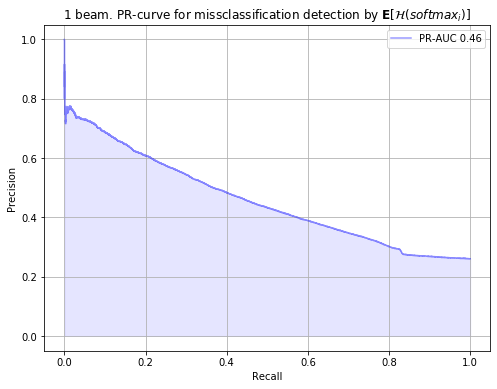
\includegraphics[width=\textwidth]{images/malinin_in_du.png}
			\center{\caption{Data uncertainty}}
		\end{subfigure}
		\center{\caption{PR-curve for misclassification detection}}
	\end{figure}
	Recall that this metric estimates knowledge uncertainty (model uncertainty). Let us take a look at experiment results for this case (figure 9(a)). As we can see $\mathbb{KL}$ solves misclassification problem worse than previous one. This results conform with the result that Malinin gets in his paper for ASR model (Knowledge uncertainty metrics estimate worse than total uncertainty estimations). Nevertheless, $\mathbb{KL}$ could be effective, if we define more resonable correctness indicator, as a total uncertainty estimation could be. 
	
	One more uncertainty estimation, that Malinin consideres in his paper is data uncertainty estimation:
	\begin{equation*}
		\mathbb{E}_{q(\theta)}[\mathcal{H}[P(y| \textbf{x}, \theta)]]
	\end{equation*}
	Expirement results, using data uncertainty estimation, are presented in figure 9(b). Obtained score is as bad as in TU case (as previous one, it conforms with Malinin ASR results). As we can see, data uncertainty estimation gains more score, than model uncertainty estimation. That is why we can suggest that, if considered metrics is resonable, so uncerainty in data influences on model prediction quality more than uncertainty in models generalization ability in ensemble.
	
	Total uncertainty, data uncertainty and knowledge uncertainty estimates low results caused by same reasons, that we discussed above. That is why let us go further.
	
	Let us now conduct similar experiments for the new correctness indicator:
	\begin{equation}
		\delta(y^i, \textbf{r}) := [y^i = r^i]
	\end{equation}
	
		
	\begin{figure}[t]
		\begin{subfigure}{.45\textwidth}
			\centering
			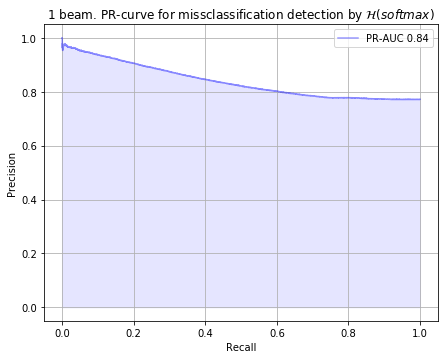
\includegraphics[width=1\textwidth]{images/malinin_eq_tu.png}
			\caption{PR-curve}
		\end{subfigure}
		\begin{subfigure}{.45\textwidth}
			\centering
			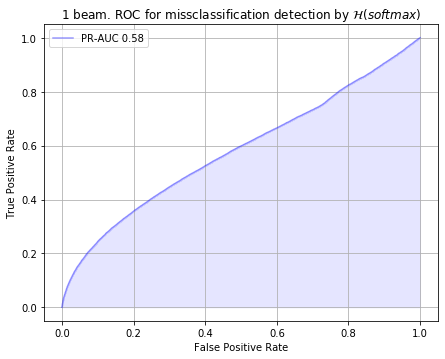
\includegraphics[width=1\textwidth]{images/malinin_eq_tu_roc.png}
			\caption{ROC}
		\end{subfigure}
		\center{\caption{Misclassification detection by TU. $\delta(y^i, \textbf{r})$}}
	\end{figure}	
	And consider the results in image 10(a). This time there are good results. However, they are not caused by the fact that we have selected a more reasonable correctness indicator, but by the fact that this indicator defines the concept of error more strictly. Now it is more likely to meet a misclassification and as a result, the uncertainty estimates have become easier to deal with this. Therefore, these results are not very reasonable. This is easy to see if we consider the ROC in image 10(b). Our empirical model does not do much better than a random algorithm. It is important to note that after we strengthened the correctness condition, the percentage of positive class increased significantly (0.76 against 0.26 in the previous statement). In this statement, we can trust ROC, since the positive class prevails and as a result, the balance of classes does not worsen experiment results.
	
	\begin{figure}[t]
		\begin{subfigure}{.45\textwidth}
			\centering
			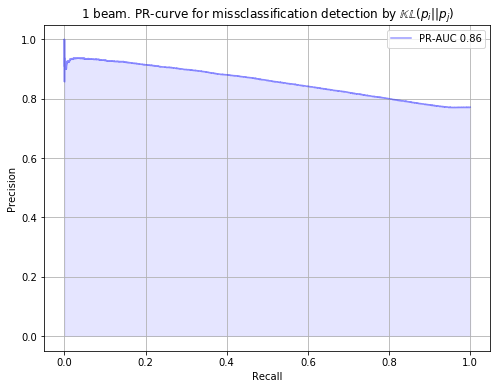
\includegraphics[width=1\textwidth]{images/malinin_eq_kl.png}
			\caption{$\mathcal{K}[y, \theta]$}
		\end{subfigure}
		\begin{subfigure}{.45\textwidth}
			\centering
			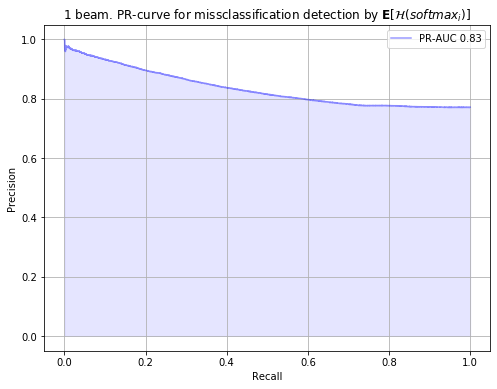
\includegraphics[width=1\textwidth]{images/malinin_eq_du.png}
			\caption{DU}
		\end{subfigure}
		\center{\caption{Misclassification detection. $\delta(y^i, \textbf{r})$}}
	\end{figure}
	
	As for previous correctness indicator, we considers data unceratainty estimate and $\mathbb{KL}$ estimate on figure 11.
	
	In all considered cases results are unreasonable. We can not trust metrics, while we use groundless correctness indicator.
	
\subsection{Experiment correctness}
	\begin{wrapfigure}{l}{0.5\textwidth}
		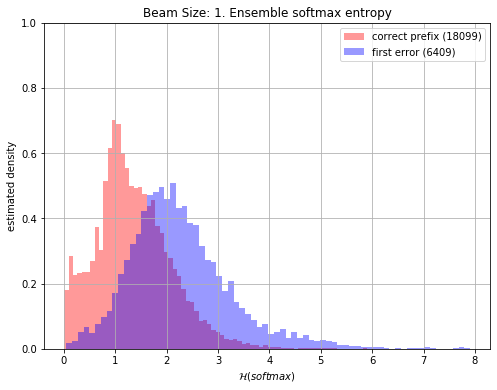
\includegraphics[width=0.5\textwidth]{images/ens_entropy.png}
		\center{\caption{Ensemble softmax Shannon entropy}}
	\end{wrapfigure}
	
	An important question arises: why a classification error can correlate with the uncertainty estimate TU.
	
	Let us try to estimate the density of the softmax entropy distribution for two cases: we correctly predict the token and we made the first error in the sentence (we predicted the entire prefix before this token correctly). In the other words, for each such case, we will calculate the softmax entropy and construct empirical density estimates (normalized histograms). The results can be seen in image 12.

	As we can see, the densities in both cases are distributed almost normally, unimodally. Moreover, the entropy distribution mode of correct tokens lies strictly to the left of the distribution mode for the first error, i.e. most of the probability mass of correct tokens has a lower softmax entropy (the TU metric).

	How can we interpret this? The higher the entropy of the distribution - the distribution is more uniform, i.e. more and more competing hypotheses appear, i.e. our ensemble identifies more and more equally probable variants, namely, less confident in its answer. Conversely, if the entropy is very low, then the distribution is close to singular, i.e. one hypothesis has about $1.$ confidence from the point of view of the ensemble.

	Thus, if the TU is large enough, it can be an indicator that we are not very confident in the token we are predicting, which allows us to estimate uncertainty in prediction.
	
	\begin{figure}[t]
		\begin{subfigure}{.45\textwidth}
			\centering
			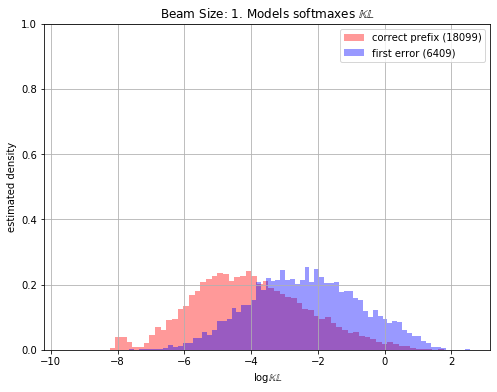
\includegraphics[width=1\textwidth]{images/ens_kl.png}
			\caption{$\mathcal{K}[y, \theta]$}
		\end{subfigure}
		\begin{subfigure}{.45\textwidth}
			\centering
			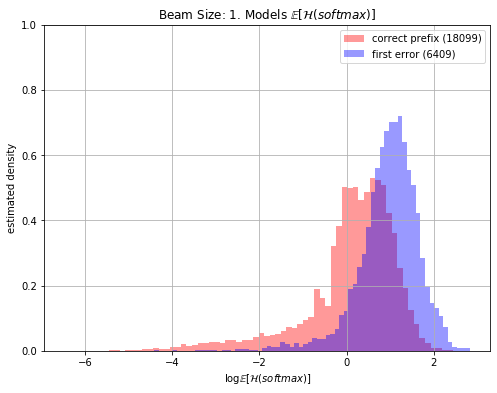
\includegraphics[width=1\textwidth]{images/ens_du.png}
			\caption{DU}
		\end{subfigure}
		\center{\caption{Uncertainty estimates distribution for correct and error tokens}}
	\end{figure}
	
	Further, let us collect same distribution but for:
	\begin{equation*}
		\mathcal{K}[y, \theta] = \mathbb{E}_{q(\theta)q(\hat{\theta})}[
			\mathrm{KL}[P(y|\textbf{x}, \theta) || P(y|\textbf{x}, \hat{\theta})
		]
	\end{equation*}
	
	Firstly, we should interpret this kind of uncertainty estimate. $\mathbb{KL}$-divergence measures difference between two distributions (more - further), this estimate is always non-negative. While we take expectation of estimate, we try to average difference between softmaxes among all possible models pairs. We can interpret $\mathcal{K}[y, \theta]$ as average value of difference between models predictions. Therefore, this metric shows us how models in ensemble conform with each other. Prerequisite to use this kind of uncertainty estimate is that it is possible, more inconsistent prediction models in ensemble make - higher probability we get to make a mistake on current token. Less formal, $\mathcal{K}[y, \theta]$ correlate with errors in predictions.
	
	Final statistics can be seen at figure 13(a). As in previous case, correct prefix density separable from first error token distribution. Moreover, expected value of kullback-leibler divergence is less than first error token's one. It meens for us, that correlation we discussed earlier exists and it could be effective to use this kind of uncertainty estimate in misclassification problem. 
	
	Our final uncertainty estimate in this section is:
	\begin{equation*}
		DU = \mathbb{E}_{q(\theta)}[\mathcal{H}[P(y| \textbf{x}, \theta)]]
	\end{equation*}
	
	As always, we should explore its meaning. While we evaluate data uncertainty estimate, we consider average single model self-confidence in ensemble. This metric is an attempt to evaluate how common considered situation ($p(y_i | y_{<i}, \textbf{x}, \theta)$) is, how presented data blends with average model generalization ability. Therefore, DU could be a good measure of data uncertainty. Prerequisite to use DU is same as previous.
	
	Final statistics for DU can be seen at figure 13(b). We can see that our prerequisite is confirmed.
	
	Overall, we considered three types of uncertainty estimation and emperically proved correlation between all types of uncertainty and predictions errors. But anyway our main barier to use uncertainty estimates in misclassification problem is token correctness indicator.
	
\subsection{Using on practice}
	Let's assume that we were able to achieve imressive results by constructing some uncertainty estimate $PerfectTU$. How can we use this to improve quality?

	Unfortunately, there are no many opportunities. All we can do is to mark positions in the sentences where we are wrong and, as a result, change our predictions. Due to the consistency of machine translation models, it would be logical to build a re-prediction not based on the original model, but to refer to some Oracle that produces more reliable predictions. In practice, such an Oracle could be some assessor or moderator. However, this approach imposes strong restrictions on the use of uncertainty estimation, since not every project can afford the support of human resources. Moreover, if you need to make fast online predictions in a task, you can no longer use moderators.

	Thus, we need to change the way we evaluate uncertainty. We need to find a way of estimating so that our model can change the predictions based on the uncertainty estimates itself. Now this is not possible, because the predicting tokens with a fixed prefix have the same uncertainty rating. As our next approach, we will not build estimates for the entire softmax at once, but for each token in the softmax separately.

	In the previous sections we have considered KL as an evaluation of knowledge uncertainty. Let us introduce a metric that will correlate with KL, but will be built for each token.
	
\subsection{Beam search}
	We conduct missclassification detection experiment for different beam size (1, 5, 9, 20, 50). We explore that for both correctness indicator with beam size growth PR-AUC degradate. It is not a significant result, because the reason of this phenomena lies in correctness indicator definition. For examle, if we consider $correct(y^i, \textbf{r})$, while beam size grows, probability to meet incorrect token in beam search grows, too, because of low positive class ratio ($~0.25$).
	
	Moreover, we do not find any correlation between beam size and uncertainty. As follow, considered uncertainty estimates can not solve larger beam size problem explicitly (in the way we do uncertainty estimation).

\section{Inensemble uncertainty estimate}
	Recall that for each token, we have denoted probability:
	\begin{equation*}
		P(y_i | y_{<i}, x, \mathcal{D}) = \frac1{K} \sum_{j=1}^{K}P(y_i | y_{<i}, x, \theta_j)
	\end{equation*}
	
	Thus, for each token, we have: a conditional probability of the token for the ensemble and K conditional probabilities of the token for the models. Let us introduce an unbiased sample variance of the token probability along the models in the ensemble as a measure of uncertainty:
	\begin{equation}
		inens\_var(y_i) := S^2(P(y_i | y_{<i}, x, \theta_1), \dots, P(y_i | y_{<i}, x, \theta_K))
	\end{equation}
	
	This estimate will serve as a measure of model consistency in predicting the probability of a given token (some analog of KL in previous chapters). Note that the entropy criterion is more suitable for us as a measure of uncertainty, since using variance it is difficult to separate cases: a singular distribution and a uniform distribution. However, variance still allows you to separate distributions with a high level of competing hypotheses. We choosed variance, because the probabilities of models do not form a probability measure (no distribution is set on these probabilities, the values may be completely inconsistent), so the calculation of entropy is incorrect in this case.
	
	\begin{figure}[t]
		\begin{subfigure}{.5\textwidth}
			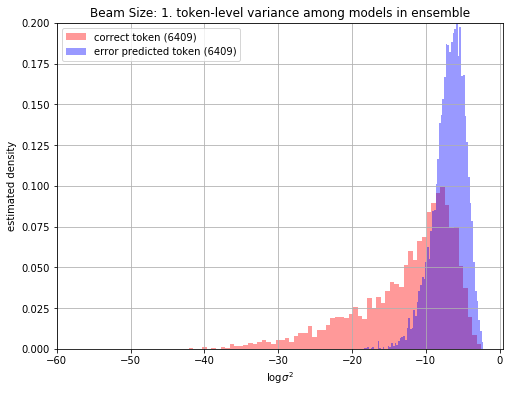
\includegraphics[width=\textwidth]{images/inens_var_density.png}
			\center{\caption{Inensemble variance among models}}
		\end{subfigure}
		\begin{subfigure}{.5\textwidth}
			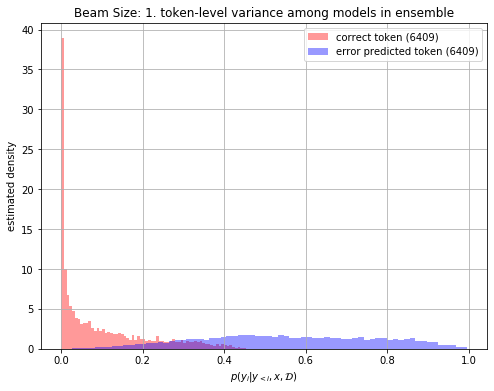
\includegraphics[width=\textwidth]{images/inens_mean_density.png}
			\center{\caption{Token probability}}
		\end{subfigure}
		\center{\caption{Statistics for correct token and first error token in softmax}}
	\end{figure}
	Consider the following graph (image 14(a)). Here is a model of a new uncertainty estimation for two types of tokens: the first false token in the prediction (the prefix before this token was predicted correctly) and the true token for this position with the same prefix. You can immediately notice that, as in the previous case, most of the probability mass of the correct token has lower variance than that of the incorrect token. This observation gives us hope that the models in the ensemble produce more consistent predictions of probabilities for the correct token and more doubt about the probability prediction for the final token.

	There is a logical question: why, despite the lower consistency, the final prediction turned out to be the token that turned out to be. To answer this question, we need to look at the probability distributions for these same tokens (image 14(b)).
	
	As we can see from the charts, we make an error in this position, because often we have about zero probability for a true token, so we prefer the more likely token (and its continuation).
	
	\begin{figure}[t]
		\begin{subfigure}{.5\textwidth}
			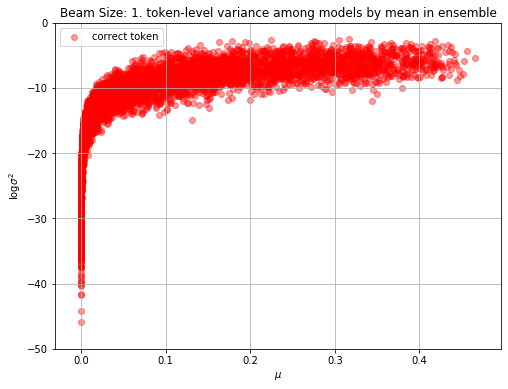
\includegraphics[width=\textwidth]{images/inens_scatter_correct.png}
			\center{\caption{Correct token}}
		\end{subfigure}
		\begin{subfigure}{.5\textwidth}
			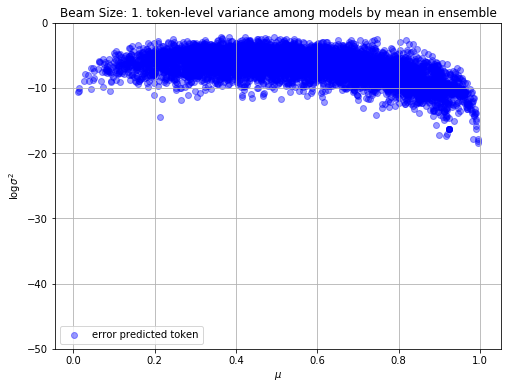
\includegraphics[width=\textwidth]{images/inens_scatter_error.png}
			\center{\caption{Error predicted token}}
		\end{subfigure}
		\center{\caption{Token-level ensemble probability by inensemble variance for correct token and first error token}}
	\end{figure}
	We would also like to see how the variance values and probability values relate to each other. Refer to figure 15. This graph reveals a serious disadvantage of considering variance. Consider the following example. Let us have some sample $t = (t_1, \dots, t_m)$ and let it correspond to the sample variance: $S^2 (t)$. Calculate:
	\begin{equation*}
		S^2(\alpha t) = S^2((\alpha t_1, \dots, \alpha t_m)) = \alpha^2 S^2(t)
	\end{equation*}
	
	Thus, the value of our metric depends not only on the total relation between values in the sample, but also on the absolute values of these values. This is the effect we saw on chart 15. For a higher probability mass of a valid token, the low value of the uncertainty estimate that we selected is not due to the consistency of the models, but rather to the values of probabilities, i.e. the variance of near zero probabilities always lower, because of property above.

	However, despite this, by comparing the variance of the correct and false token with equal probabilities, we can observe that the expected variance for the correct token is lower than for the false one. Therefore, although not on the entire probability mass, but on some of its part, our estimation of uncertainty gives adequate predictions.

	In order to make sure of this, you need to see how our rating behaves on other tokens of the same softmax. To do this, we will consider: a random token, tokens with top-3, top-5, and top-20 probabilities in a descending series of variations. The final graphs of the probability distribution and uncertainty estimates can be seen in figure 16.
	
	As we can see, correct tokens are not so hopeless. A high proportion of the probability mass of correct tokens has relatively high probabilities (the expected position in the variation series of probabilities == 2). Moreover, the models ' confidence in the correct tokens is not inferior to the variance of other tokens. We can use these observations to help the model find the correct tokens.
	
	\begin{figure}[H]
		\center{
			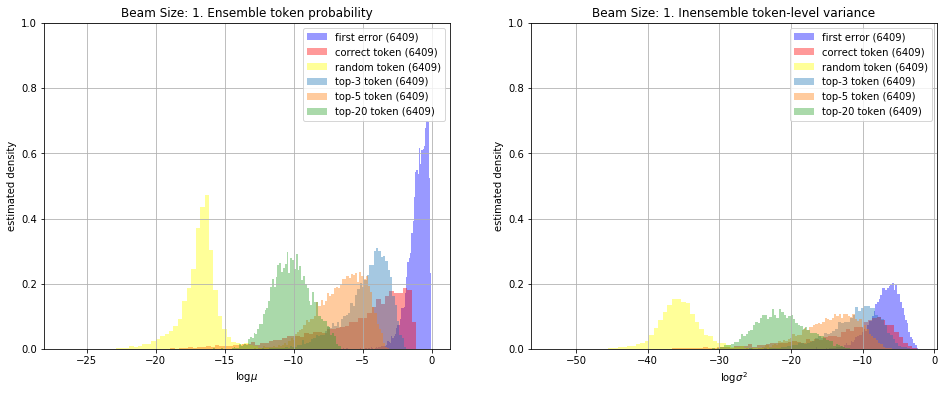
\includegraphics[width=\textwidth]{images/inens_stats_top.png}
		}
		\center{\caption{Token-level ensemble probability and inensemble variance for correct token, first error token, random token, top-3 top-5 and top-20 tokens}}
	\end{figure}
	
\subsection{Probability distribution calibration}
	Our task now is to renormalize the probability distributions of tokens with the uncertainty metric in such a way that the distribution of the correct token becomes more prevalent in terms of choosing the final hypothesis by the model. Thus, the problem is reduced to finding some function $g$:
	\begin{equation*}
		\hat{p}(y | x, \mathcal{D}) = softmax(g(p(y | x, \mathcal{D}),\, inens\_var(y)))
	\end{equation*}
	
	If we look at graph 17, it becomes clear that by selecting $g$, we can only bend this graph along the x axis. In visual terms, we would like to pull the density of the correct token to the right edge along each contour line of the variance, and the density of any other token to the left.
	
	\begin{figure}[t]
		\center{
			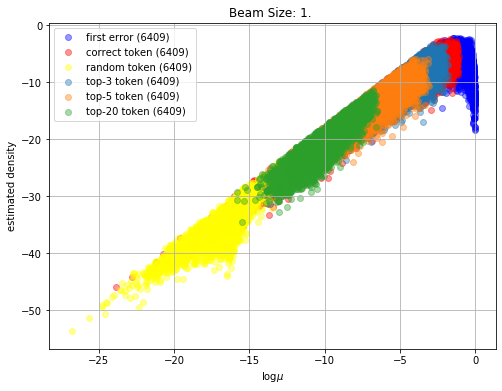
\includegraphics[width=0.6\textwidth]{images/calibration_baseline_scatter.png}
		}
		\center{\caption{Token-level ensemble probability by inensemble variance for correct token, first error token, random token, top-3 top-5 and top-20 tokens}}
	\end{figure} 
	
	Remind that we want to penalize for high values of uncertainty, but not so much as to overweight completely irrelevant tokens. A bad example of the $g$ function would be:
	
	Here and further, let us denote: $\sigma^2 := inens\_var$
	\begin{equation}
		g_{naive} := \log p(y | x, \mathcal{D}) - \log(\sigma^2)
	\end{equation}
	
	We explicitly reward tokens with a very low variance value and, conversely, heavily penalize them for high uncertainty values. This naive approach leads to a diametrically opposite situation that we want to get (image 18(a)). We can see that such strong penalties lead to a high probability of accepting random tokens. This is because the variance of random tokens is extremely low due to the property of the variance that we discussed earlier. As a result, the model simply produces completely random translations.
	
	\begin{figure}[t]
		\begin{subfigure}{.5\textwidth}
			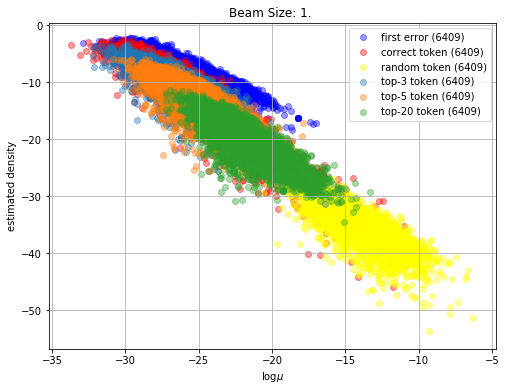
\includegraphics[width=\textwidth]{images/calibration_naive_scatter.png}
			\center{\caption{$g = g_{naive}$}}
		\end{subfigure}
		\begin{subfigure}{.5\textwidth}
			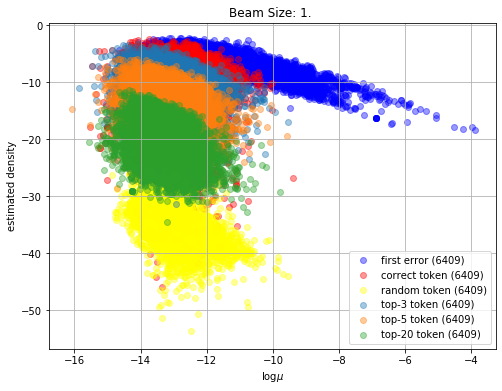
\includegraphics[width=\textwidth]{images/calibration_lessnaive_scatter.png}
			\center{\caption{$g = g_{less\_naive}$}}
		\end{subfigure}
		\center{\caption{Token-level ensemble probability by inensemble variance for correct token, first error token, random token, top-3 top-5 and top-20 tokens for $g$}}
	\end{figure}
	
	Let us try to slightly weaken the penalty for uncertainty, divide the probability by the root of the variance:
	\begin{equation}
		g_{less\_naive} := \log p(y | x, \mathcal{D}) - \log(\sigma)
	\end{equation}
	
	As we can see from graph 18(b), this did not bring any success, since we did not even change the relative order of probability distributions.

	If we take another look at graph 17, it will be clear that we cannot use linear functions $g$ to rearrange the order of distributions in terms of probabilities (recall that the graph is presented in log scales). Thus, we come to the conclusion that the calibration must not be linear by $\log \sigma^2$, moreover, the peak (maximum point) must fall on a part of the distribution of the correct token, which is not overlapped by any other distribution.

	Then let us take a function:
	\begin{equation}
		g_{2} := \log p(y | x, \mathcal{D}) - (\log(\sigma) + \alpha)^2
	\end{equation}
	
	 Where $\alpha$ is a certain hyperparameter that will depend on which point the maximum will be reached. Let us consider a special example (graph 19(a)).
	\begin{figure}[t]
		\begin{subfigure}{.5\textwidth}
			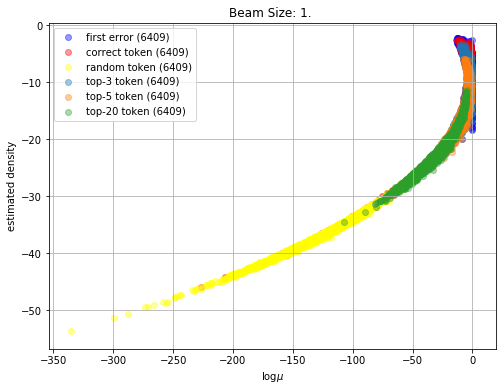
\includegraphics[width=\textwidth]{images/calibration_g2_scatter.png}
			\center{\caption{Calibrated probabilities by variance}}
		\end{subfigure}
		\begin{subfigure}{.5\textwidth}
			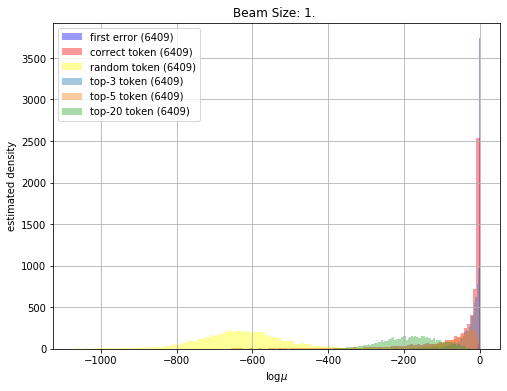
\includegraphics[width=\textwidth]{images/calibration_g2_probs.png}
			\center{\caption{Calibrated probabilities histogram}}
		\end{subfigure}
		\center{\caption{$g_2$ statistics for correct token, first error token, random token, top-3 top-5 and top-20 tokens. \\
		$g_2 = \log p(y | x, \mathcal{D}) - (\log(\sigma) + 4)^2$}}
	\end{figure}
	
	As we can see, now most probability mass of correct token moved forward to first positions in probability variational series, but also top tokens moved forward too. By the reason of fact, all tokens' distributions are mixed, we can not certainly separate correct token distribution from any other. But we can make correct token more prevailing over any other token on a fixed variance counter level. As we can see on a chart, we achieve this goal.
	
	Note that the density of the wrong token still remains to the right of the density of the correct token. Unfortunately or fortunately, we can't do anything with these points, because if a certain token has a high probability on the same contour line of variance, obviously, we should give preference to this particular token. However, even this results can lead to good results, because in the case of a non-single beam size, even a small overweight can lead to the choice of correct hypotheses, because the choice of hypothesis is based on cumulative probabilities, not on a greedy choice.
	
	If we take a look at figure 19(b), we can see ensemble probability distributions after $g_2$ calibration. Our hypothesis about correct token prevailation confirms.
	
	An important note about results is that, while we use beam search with beam size equal $1$, we will not earn better results using $g_2$ calibration, because most part of first error token is still most probable. But if we consider beam search model with beam size more than $1$, we can expect quality improvement, because non-greedy beam search not always chooses most likely token and estimate next token probability using cumulative prefix probability.

\subsection{Calibration BLEU}
	Let us consider BLEU4 evaluation on a test set for calibrated ensemble (figure 20).
	
	\begin{figure}[t]
		\begin{subfigure}{.5\textwidth}
			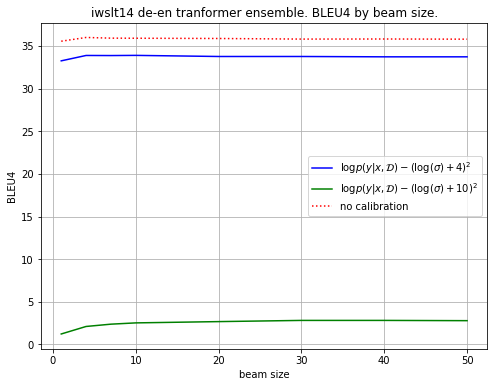
\includegraphics[width=\textwidth]{images/calibratin_bleu_all.png}
			\center{\caption{}}
		\end{subfigure}
		\begin{subfigure}{.5\textwidth}
			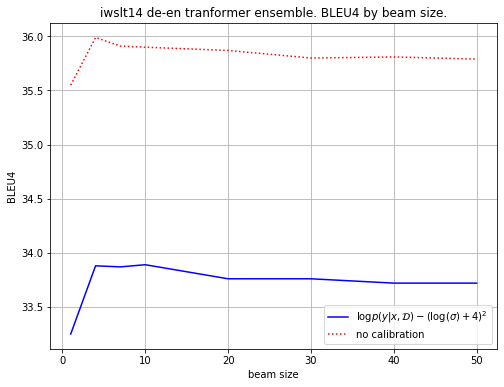
\includegraphics[width=\textwidth]{images/calibration_bleu_best.png}
			\center{\caption{}}
		\end{subfigure}
		\center{\caption{BLEU4 by beam size for calibrated transformer ensemble}}
	\end{figure}
	
	\begin{figure}[t]
		\begin{subfigure}{.5\textwidth}
			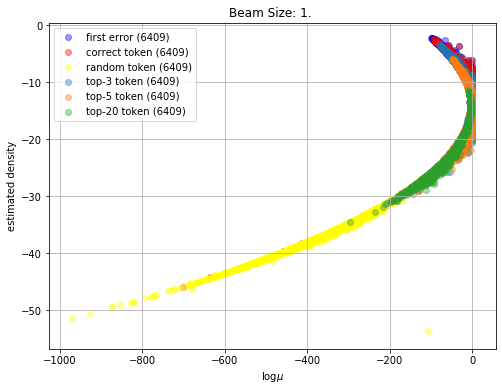
\includegraphics[width=\textwidth]{images/calibration_g10_scatter.png}
			\center{\caption{Calibrated probabilities by variance}}
		\end{subfigure}
		\begin{subfigure}{.5\textwidth}
			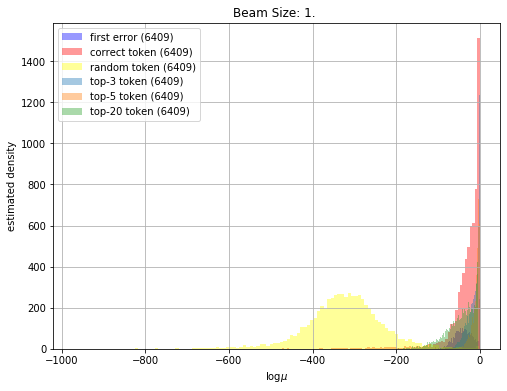
\includegraphics[width=\textwidth]{images/calibration_g10_probs.png}
			\center{\caption{Calibrated probabilities histogram}}
		\end{subfigure}
		\center{\caption{$g_2$ statistics for correct token, first error token, random token, top-3 top-5 and top-20 tokens. \\
		$g_2 = \log p(y | x, \mathcal{D}) - (\log(\sigma) + 10)^2$}}
	\end{figure}
	
	As we can see, baseline ensemble without any calibration overperforms all our tested calibrated models. The worst results are presented by square calibration with bias equal $10$. BLEU is less than 5 for this case. The reason of this poor results can be seen at figure 21. After calibration all top-20 (including all more probable tokens) mix together that is why in lots of cases softmaxes have more entropy (recall it meens that our model more uncertain in predictions), so we get a lot of more random predicted tokens. The problem is we choose bias too large and calibration scatter peak is not on correct token distribution but on irrelevant tokens (top-5 top-20 tokens). Therefore, we get too low BLEU.
	
	More significant results are presented by calibration with bias equal $4$. The problem in this case is similar to previous one. Now peak is placed on more relevant tokens, but still irrelevant (top-3) tokens enter in resulting predictions. Therefore, let us conduct same experiment but with less bias.
	
	\textbf{TODO Bias == 1.1}
	
	Overall, we consider different kinds of calibration, but we did not achieve quality improvement. The reason of poor final results lie on a weak uncertainty estimate. If we look at figure 16, we can see that inensemble variance distribution for correct token overlap all tokens distributions (except random one) that is why, it is too hard to separate correct token from others. Too small part of correct token distribution for variance is separable from others. This part is too small to get enough quality improvement.
\section{Conclusion}
	In this work we conduct misclassification detection experiments, using different types of uncertainty estimates, on neural machine translation task. We explore correlation between uncertainty and predictions error, analysing uncertainty estimates distributions. Our conclusion is that it is possible to detect prediciton error via uncertainty estimation, because considered uncertainty estimates correlate with errors (correct tokens have lower expected values than others). At the same time, it is hard to evaluate correct quality estimation for misclassification detection via uncertainty, because there are lots of problems with defining reasonable tokens correctness measure.
	
	Moreover, we go deeper softmax level and explore new way of uncertainty estimation. We introduce inensemble uncertainty estimate for every token. We approve correlation between new measure and predictions error. As well, we try to recalibrate token probabilities using token-level inensemble varinace.
	
	Unfortunately, we do not achive model quality improvement, but also we do not claim that this hypothesis is wrong. Further studies should conduct same experiments using different uncertainty estimates. As we conclude inensemble variance distribution has weak correlation with error predictions to achive high quality improvement.
	
	\begin{thebibliography}{0}		
		\bibitem{fconv}\hypertarget{fconv}{}
		\href{https://arxiv.org/pdf/1705.03122.pdf}
		{Jonas Gehring, Michael Auli, David Grangier, Denis Yarats, Yann N. Dauphin. Facebook AI Research. Convolutional Sequence to Sequence Learning. PMLR 70, 2017.}
		
		\bibitem{seq2seq}\hypertarget{seq2seq}{}
		\href{https://papers.nips.cc/paper/5346-sequence-to-sequence-learning-with-neural-networks.pdf}
		{Ilya Sutskever, Oriol Vinyals, Quoc V.Le. Sequence to Sequence Learning with Neural Networks. Google. NIPS 2014.}
		
		\bibitem{encdec_att}\hypertarget{encdec_att}{}
		\href{https://arxiv.org/pdf/1409.0473.pdf}
		{Dzmitry Bahdanau, KyungHyun Cho, Yoshua Bengio. Neural Machine Translation by Jointly Learning to Align and Translate. ICLR 2015.}
		
		\bibitem{corr_len_bias}\hypertarget{corr_len_bias}{}
		\href{https://arxiv.org/pdf/1808.10006.pdf}
		{Kenton Murray, David Chiang. Department of Computer Science and Engineering, University of Notre Dame. Correcting Length Bias in Neural Machine Translation. WMT 2018.}
		
		\bibitem{gnmt}\hypertarget{gnmt}{}
		\href{https://arxiv.org/pdf/1609.08144.pdf}
		{Yonghui Wu, Mike Schuster, Zhifeng Chen, Quoc V. Le, Mohammad Norouzi. Google’s Neural Machine Translation System: Bridging the Gapbetween Human and Machine Translation. ArXiv 2016}
		
		\bibitem{transformer}\hypertarget{transformer}{}
		\href{https://arxiv.org/pdf/1706.03762.pdf}
		{Ashish Vaswani, Noam Shazeer, Niki Parmar, Jakob Uszkoreit, Llion Jones, Aidan N. Gomez, Lukasz Kaiser. Attention Is All You Need. NIPS 2017.}
		
		\bibitem{six_chall}\hypertarget{six_chall}{}
		\href{https://arxiv.org/pdf/1706.03872.pdf}
		{Philipp Koehn, Rebecca Knowles. Six Challenges for Neural Machine Translation. NMT@ACL 2017.}
		
		\bibitem{calibration}\hypertarget{calibration}{}
		\href{https://arxiv.org/pdf/1903.00802v1.pdf}
		{Aviral Kumar, Sunita Sarawagi. Calibration of Encoder Decoder Models for Neural Machine Translation. ArXiv 2019.}
		
		\bibitem{anal_uncertainty}\hypertarget{anal_uncertainty}{}
		\href{https://arxiv.org/pdf/1803.00047.pdf}
		{Myle Ott, Michael Auli, David Grangier, Marc'Aurelio Ranzato. Analyzing Uncertainty in Neural Machine Translation. PMLR 80, 2018.}
		
		\bibitem{prior}\hypertarget{prior}{}
		\href{https://papers.nips.cc/paper/7936-predictive-uncertainty-estimation-via-prior-networks.pdf}
		{Andrey Malinin, Mark Gales. Predictive Uncertainty Estimation via Prior Networks. NeurIPS 2018.}
		
		\bibitem{uncertainty}\hypertarget{uncertainty}{}
		\href{https://arxiv.org/pdf/2002.07650.pdf}
		{Andrey Malinin, Mark Gales. Uncertainty in Structured Prediction. 2020.}
	\end{thebibliography}


\end{document}

